\chapter{Algnment Examples}\label{appendix-a}

I would like to shortly compare the  alignments computed by eflomal and SimAlign (mBERT, subword level, Itermax method, cf., Sections~\ref{subsec:simalign-method} and~\ref{sec:performance-simalign}) with my annotations from the gold standard, especially regarding some of the examples I mentioned in Chapter~\refnameref{chap:gold-standard} for handling ambiguous cases.
I will consider the following cases: German compounds,  German preterite and perfect vs.~Romansh perfect and Romansh double negation. 
Please refer to Section~\ref{sec:gold-standard-examples}: Gold Standard--Examples for more details.

In all of the examples below, \textbf{filled green squares} are the \textbf{gold standard},\textbf{ circles} are alignments produced by \textbf{SimAlign} and \textbf{boxes} are alignments produced \textbf{eflomal}. 

The plots were created using a script provided on GitHub\footnote{\url{https://github.com/cisnlp/simalign/blob/master/scripts/visualize.py}} accompanying SimAlign \autocite{jalili-sabet-etal-2020-simalign}.

\section{Compounds}
First, I would like to see how eflomal and SimAlign deal with aligning German compounds.

eflomal seems to be doing a better job creating 1-to-many alignments for compounds. 
In Figure~\ref{fig:die-ostschwizer-fachhochschule}, eflomal aligns  the German word \emph{Fachhochschule} (\emph{technical college}) correctly  to Romansh \emph{Scola auta spzialisada}, whereas SimAlign only aligns it to \emph{Scola} (\enquote{school}). 
However, both models correctly align German \emph{Ostschweizer} (\enquote{eastern Swiss}) to Romansh \emph{Svizra Oreintala}.

Figure~\ref{fig:ergaenzend} shows a similar case. The German compound \emph{Grundversorgungsauftrag} (\enquote{basic services mission}) is aligned by eflomal to two words in Romansh: \emph{incumbensa} and \emph{provediment}. But it leaves \emph{basa} wrongly unaligned. 
The compound \emph{Nationalstrassen} (\enquote{national roads}) is correctly aligned to \emph{vias naziunalas} by eflomal. SimAlign again only aligns the first word of the corresponding Romansh words: \emph{incumbensa}  and \emph{vias}, respectively.

In yet another case (Figure~\ref{fig:das-leitbild}), both models succeed in creating a 1-to-2 alignment by aligning the German word \emph{Leitbild} (\enquote{role model}) to Romansh \emph{model directiv}. 
However, eflomal fails to align German \emph{departmentsübergreifend} (\enquote{inter-departmental}) to Romansh \emph{interdepartamental}, although this would have been a 1-to-1 alignment. I am assuming that this is due to this word appearing only once in the entire corpus. 
SimAlign succeeds here, probably due to these words (or parts of them) having appeared enough times in the monolingual training data of mBERT. 
The German compound \emph{Aufgabenfeld} (\enquote{field of duties}) is aligned by SimAlign only to the first word again: \emph{champ} (\enquote{field}). 
eflomal fails here completely.


To summarize, it seems eflomal generally does a better job creating 1-to-many alignments for German compounds. 
However, a much larger sample size would be needed to reach definite conclusions.

\begin{figure}
	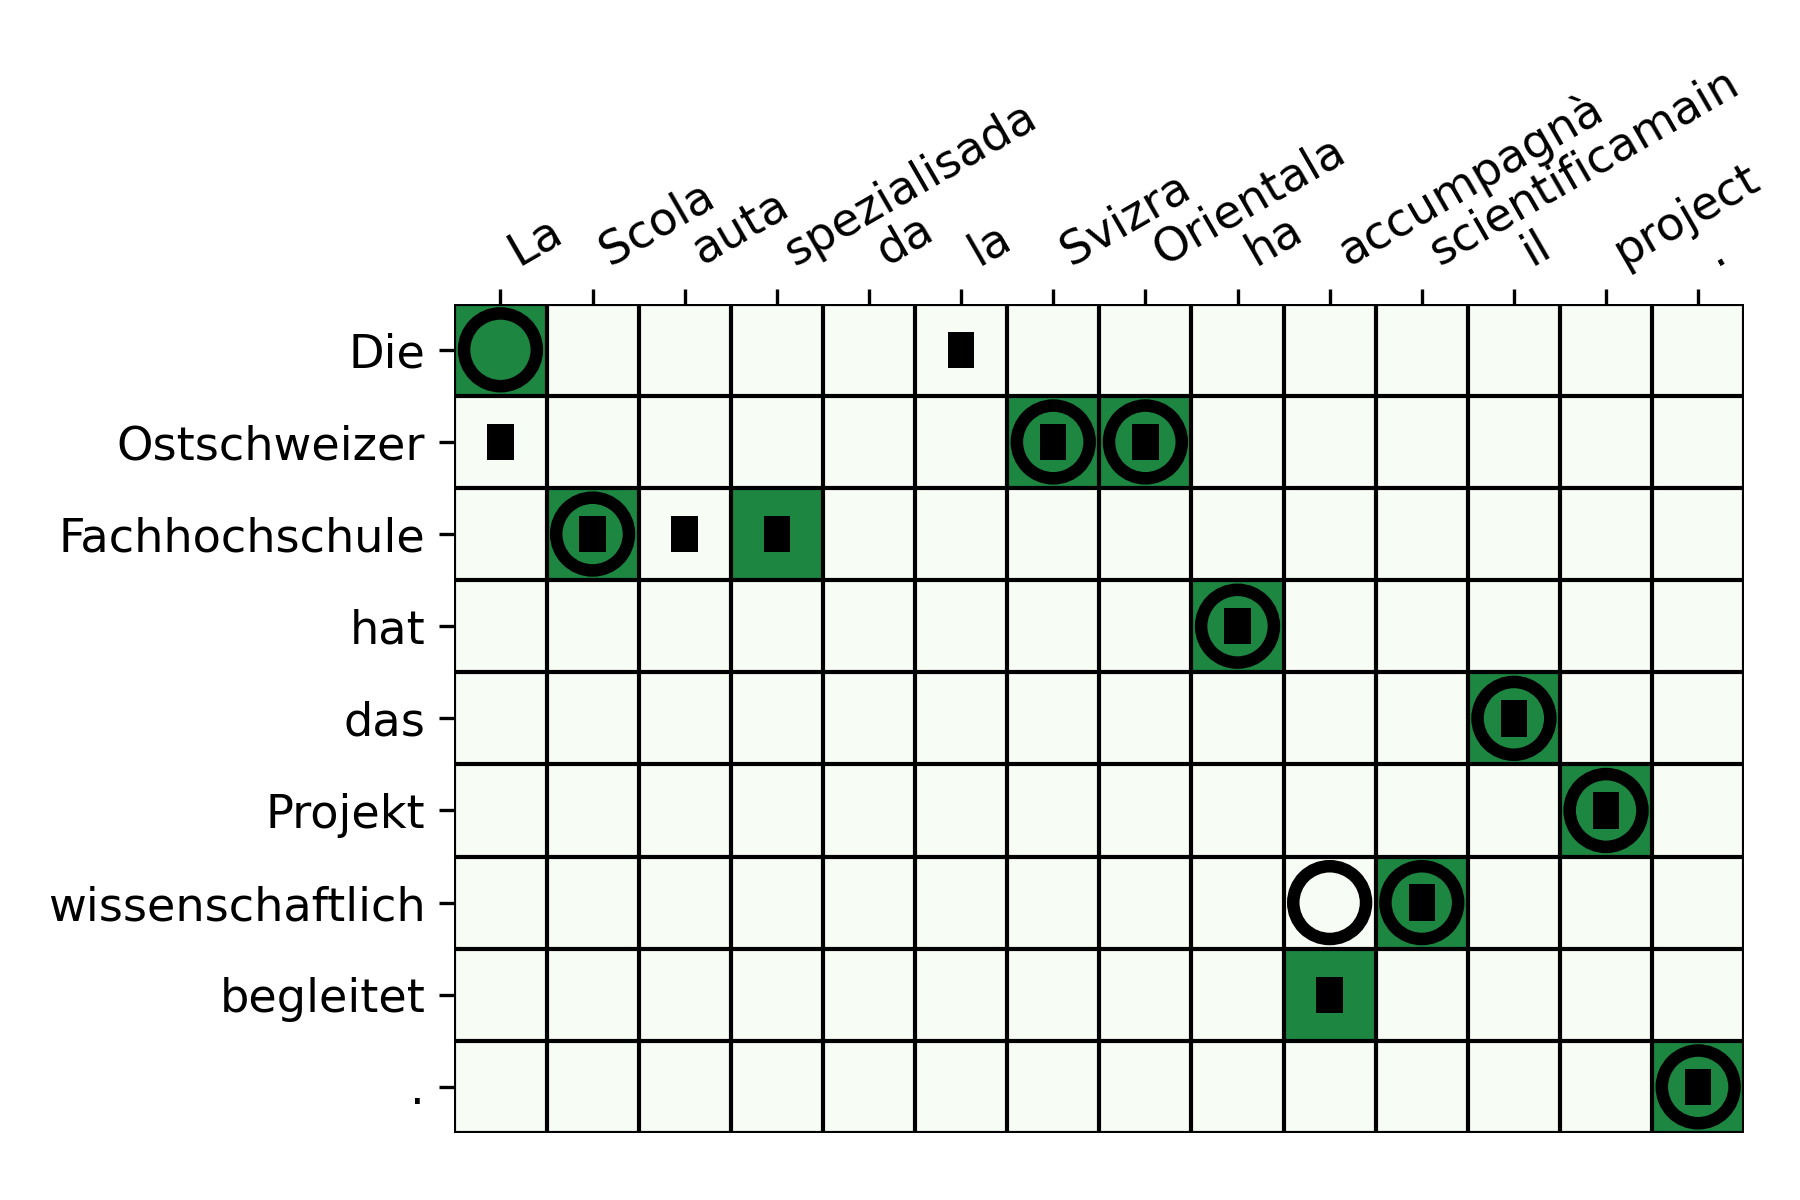
\includegraphics{graphics/alignments/example7-prefect2.png}
	\caption{Word alignment example for the case of perfect tense in German and Romansh}\label{fig:die-ostschwizer-fachhochschule}
\end{figure}

% \begin{figure}
% 	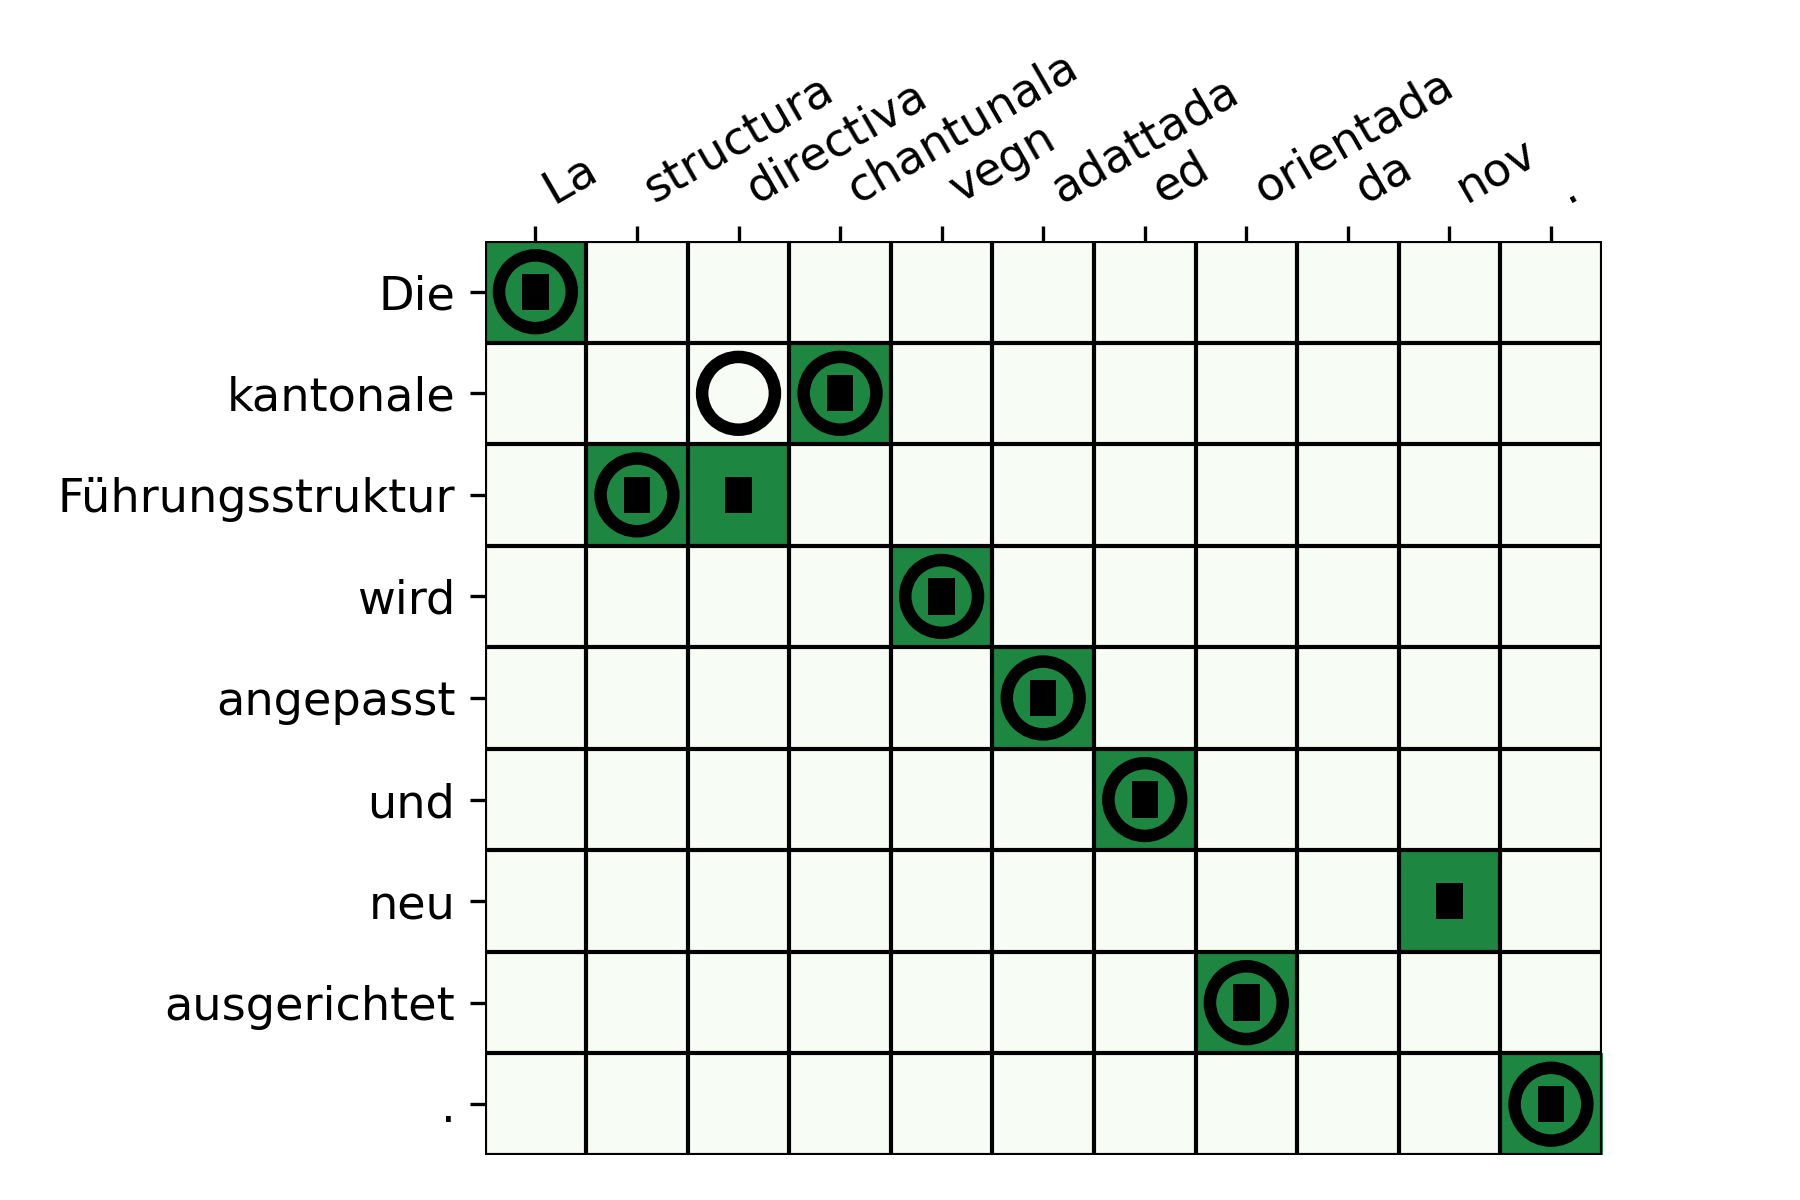
\includegraphics{graphics/alignments/example4.png}
% 	\caption{Word alignment example containing a compound and two participles.}
% 	\label{fig:die-kantonale-fuehrung} 
% \end{figure}


\begin{figure}
	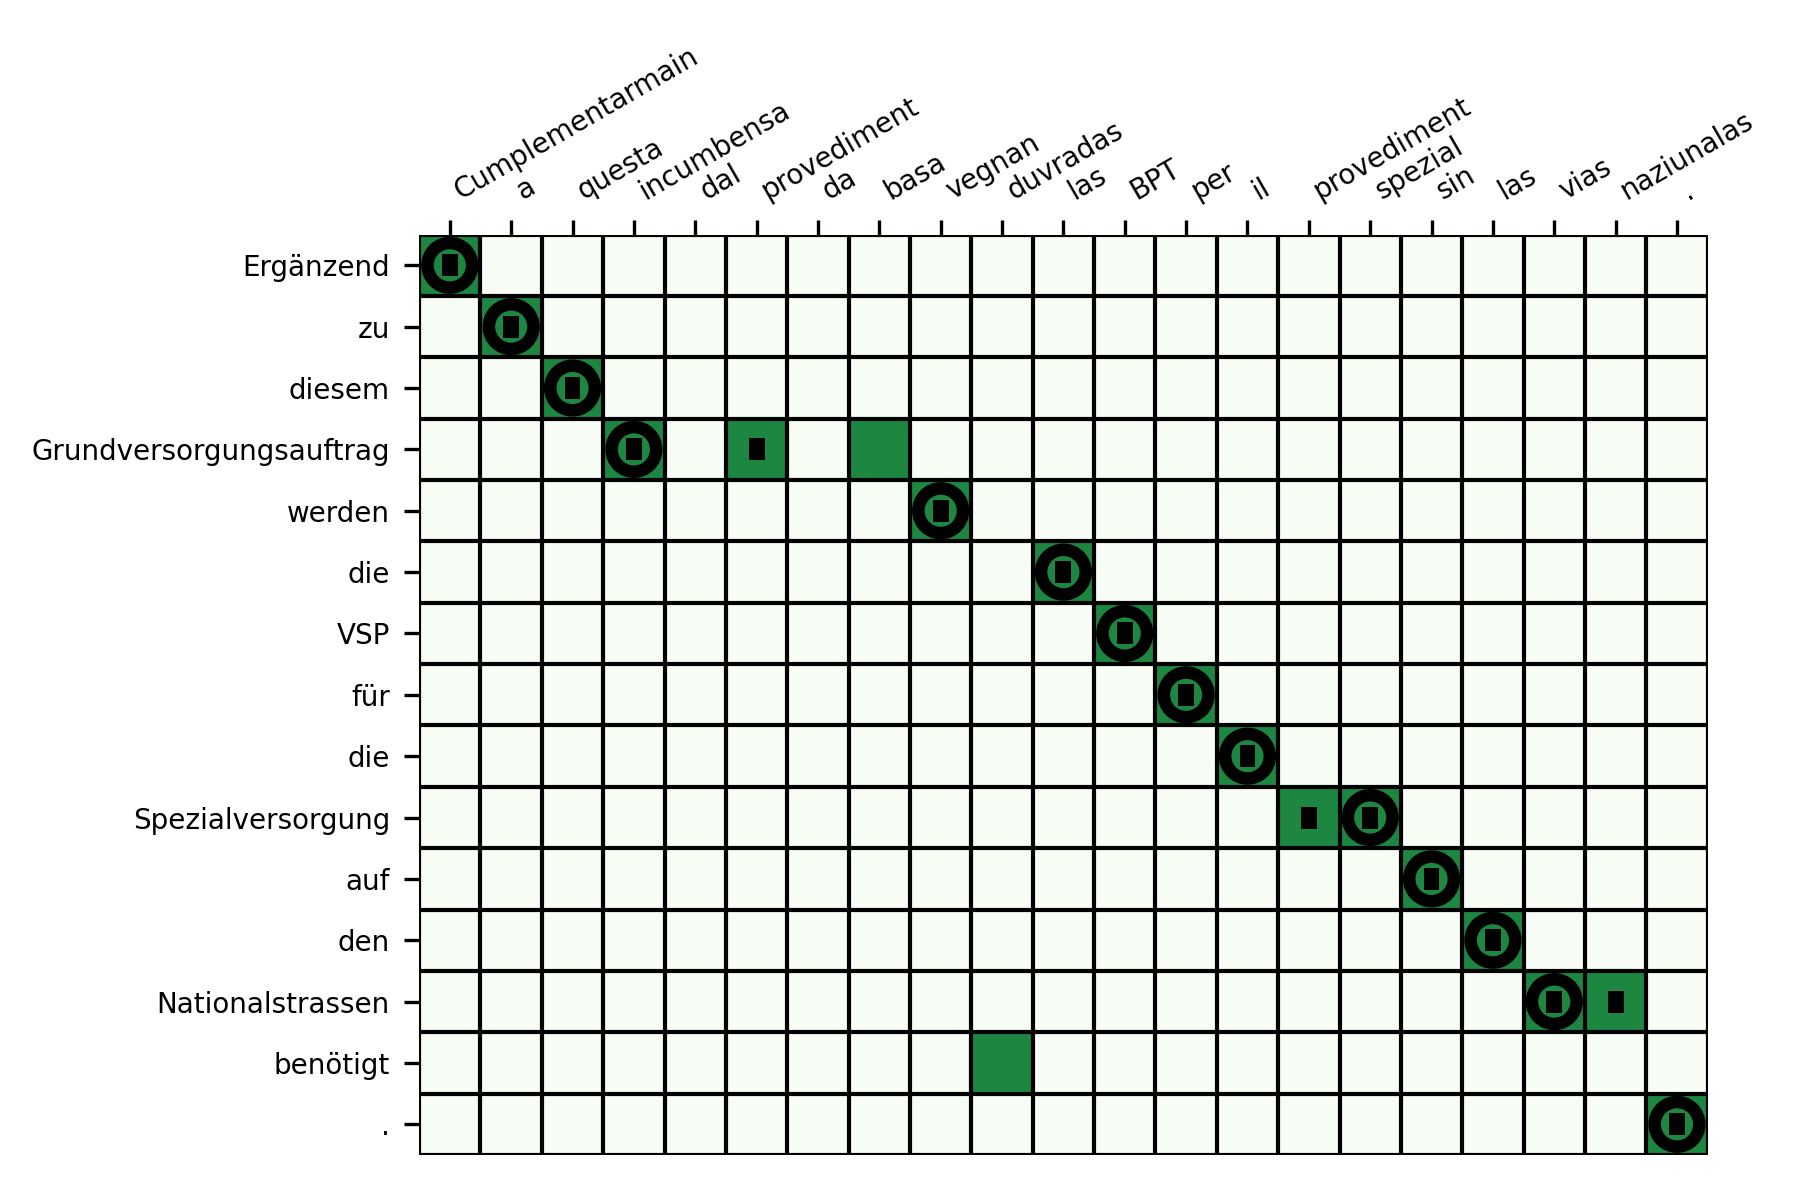
\includegraphics{graphics/alignments/compounds1.png}
	\caption{Word alignment example with compounds.}
	\label{fig:ergaenzend}
\end{figure}

\begin{figure}
	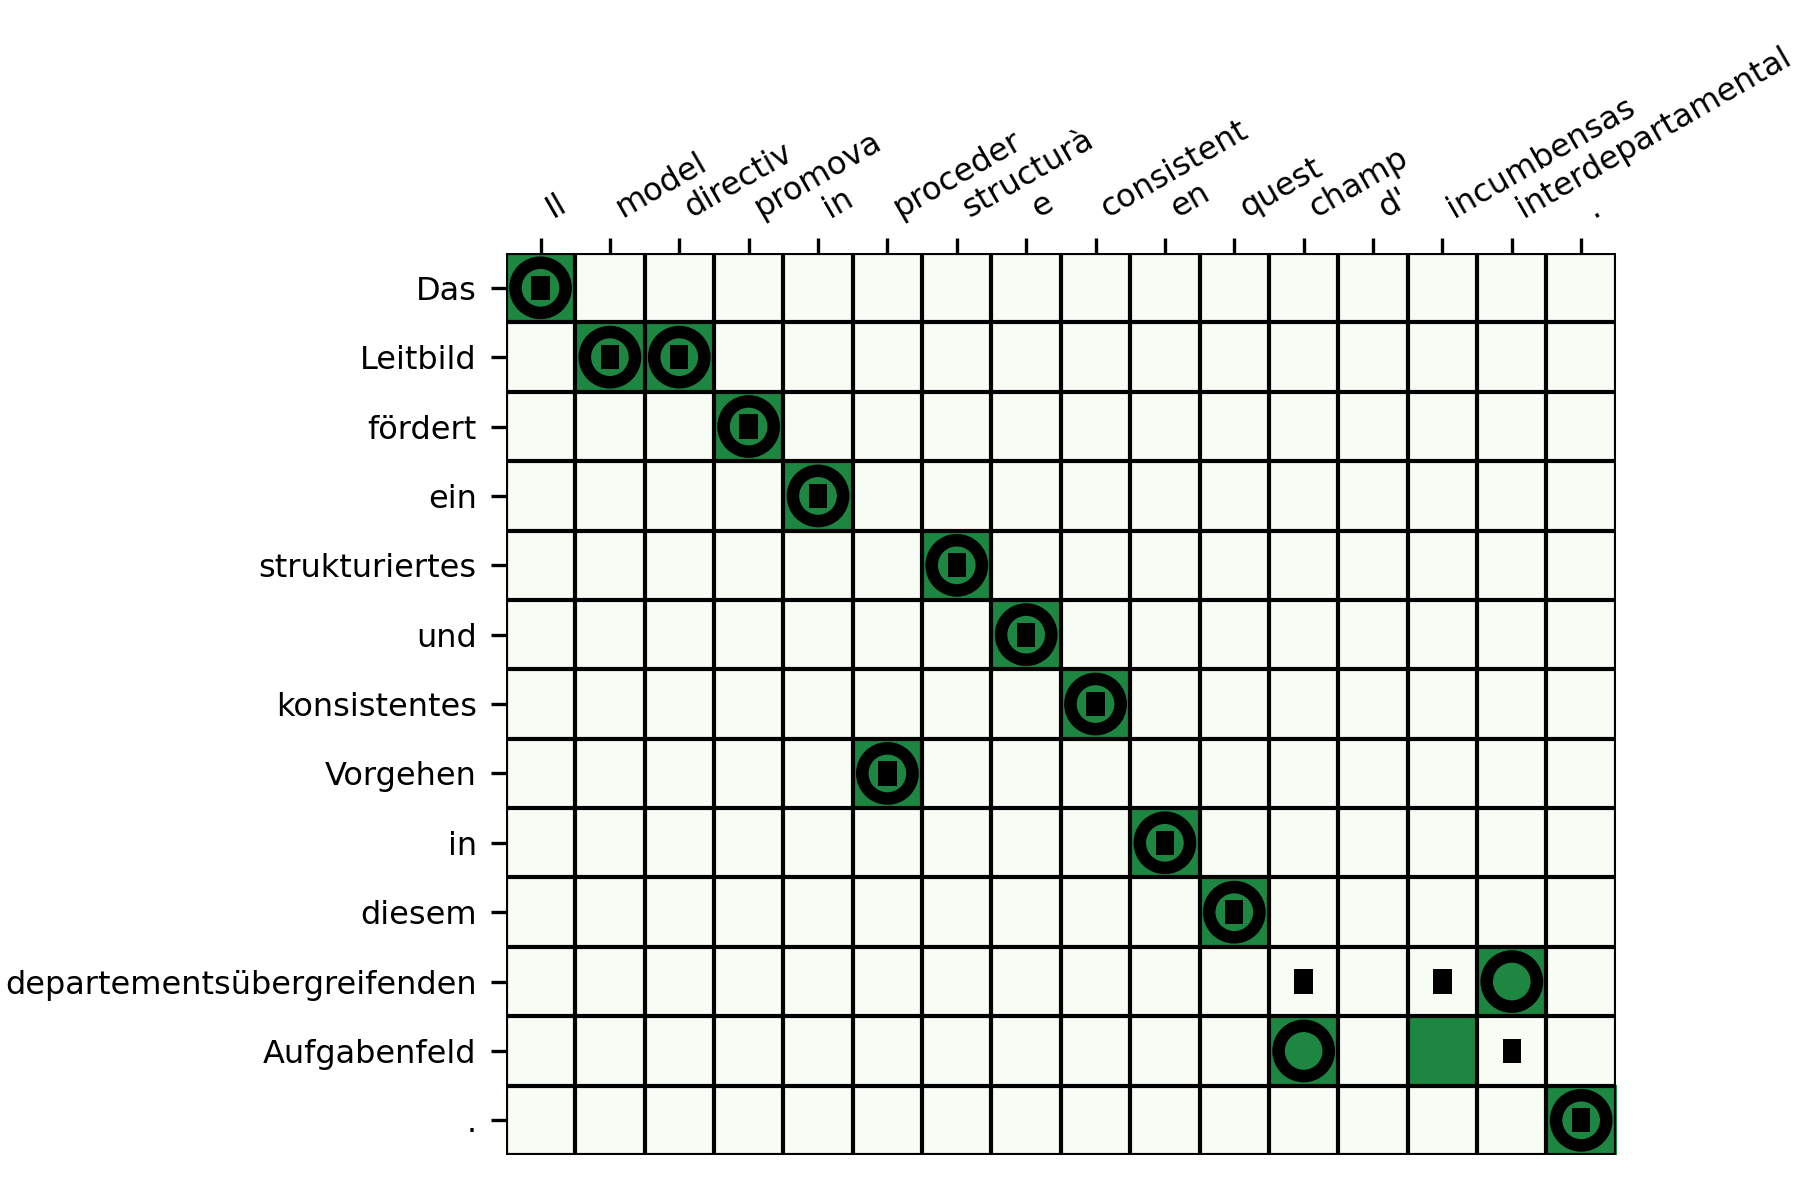
\includegraphics{graphics/alignments/compounds2.png}
	\caption{Word alignment example with compounds.}
	\label{fig:das-leitbild}
\end{figure}




\section{Perfect--Perfect}\label{sec:perfect-perfect}
Figure~\ref{fig:die-regierung} shows an example for aligning the German perfect with the Romansh perfect. 
The German and the Romansh auxiliaries \emph{hat} and \emph{ha} should be aligned to each other, as well as the German and the Romansh participles \emph{verabschiedet} and \emph{deliberà}. 
SimAlign's alignment are in accord with the gold standard, while eflomal aligned Romansh \emph{deliberà} to German \emph{hat}, leaving German \emph{verabschiedet} unaligned. However, in another case (Figure \ref{fig:die-ostschwizer-fachhochschule}), eflomal correctly aligned the German participle to the Romansh participle, whereas SimAlign didn't. 
It would be interesting to test this on a larger scale and see which system is more consistent regarding this.

\begin{figure}
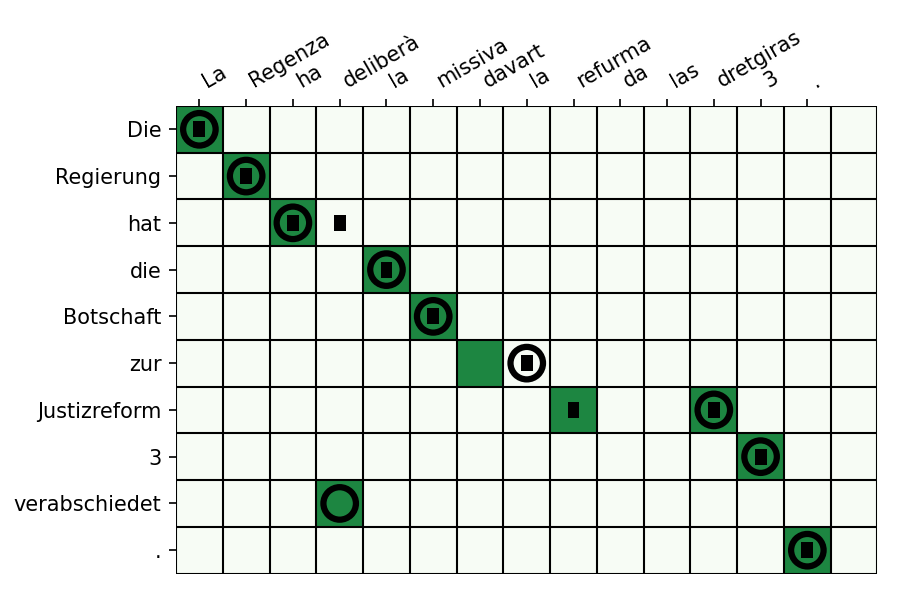
\includegraphics{graphics/alignments/example1.png}
\caption{Word alignment example for the case of perfect tense in German and Romansh}\label{fig:die-regierung}
\end{figure}





\section{German Preterite--Romansh Perfect}

In the matter of aligning the German preterite with Romansh perfect, eflomal creates a 1-to-2 alignment, connecting both the auxiliary \emph{han} and the participle \emph{visità} to the German preterite \emph{besichtigten} (Example~\ref{fig:pret1}), an alignment which is not even acceptable, but also desirable, but which I chose to avoid in my annotations due to my preference of 1-to-1 alignments. However, in a different case (Example~\ref{fig:pret2}), eflomal failed to align the participle, which is lexically the more important part, and left it unaligned . 
SimAlign successfully aligns the German preterite to the Romansh participle in the first case, but fails as well in the second case.
In the case of preterite--perfect, there is no clear advantage of any of the models over the other.

Example~\ref{fig:109-1912-nahm} presents an even more challenging case. 
Here we are dealing with a separable German verb in preterite \emph{nahm ... 
auf} (\enquote{start, open}) , which is translated to the Romansh perfect \emph{ha ...~avert} (\enquote{has ... 
opened}). 
The gold standard stipulates that German \emph{nahm ... 
auf} should be aligned to Romansh \emph{avert}, leaving the Romansh auxiliary \emph{ha} unaligned. 
However, both models align German \emph{nahm} to Romansh \emph{ha}. SimAlign leaves \emph{avert} completely unaligned; eflomal aligns \emph{avert} to \emph{Gebäudeversicherung}, which is wrong.

\begin{figure}
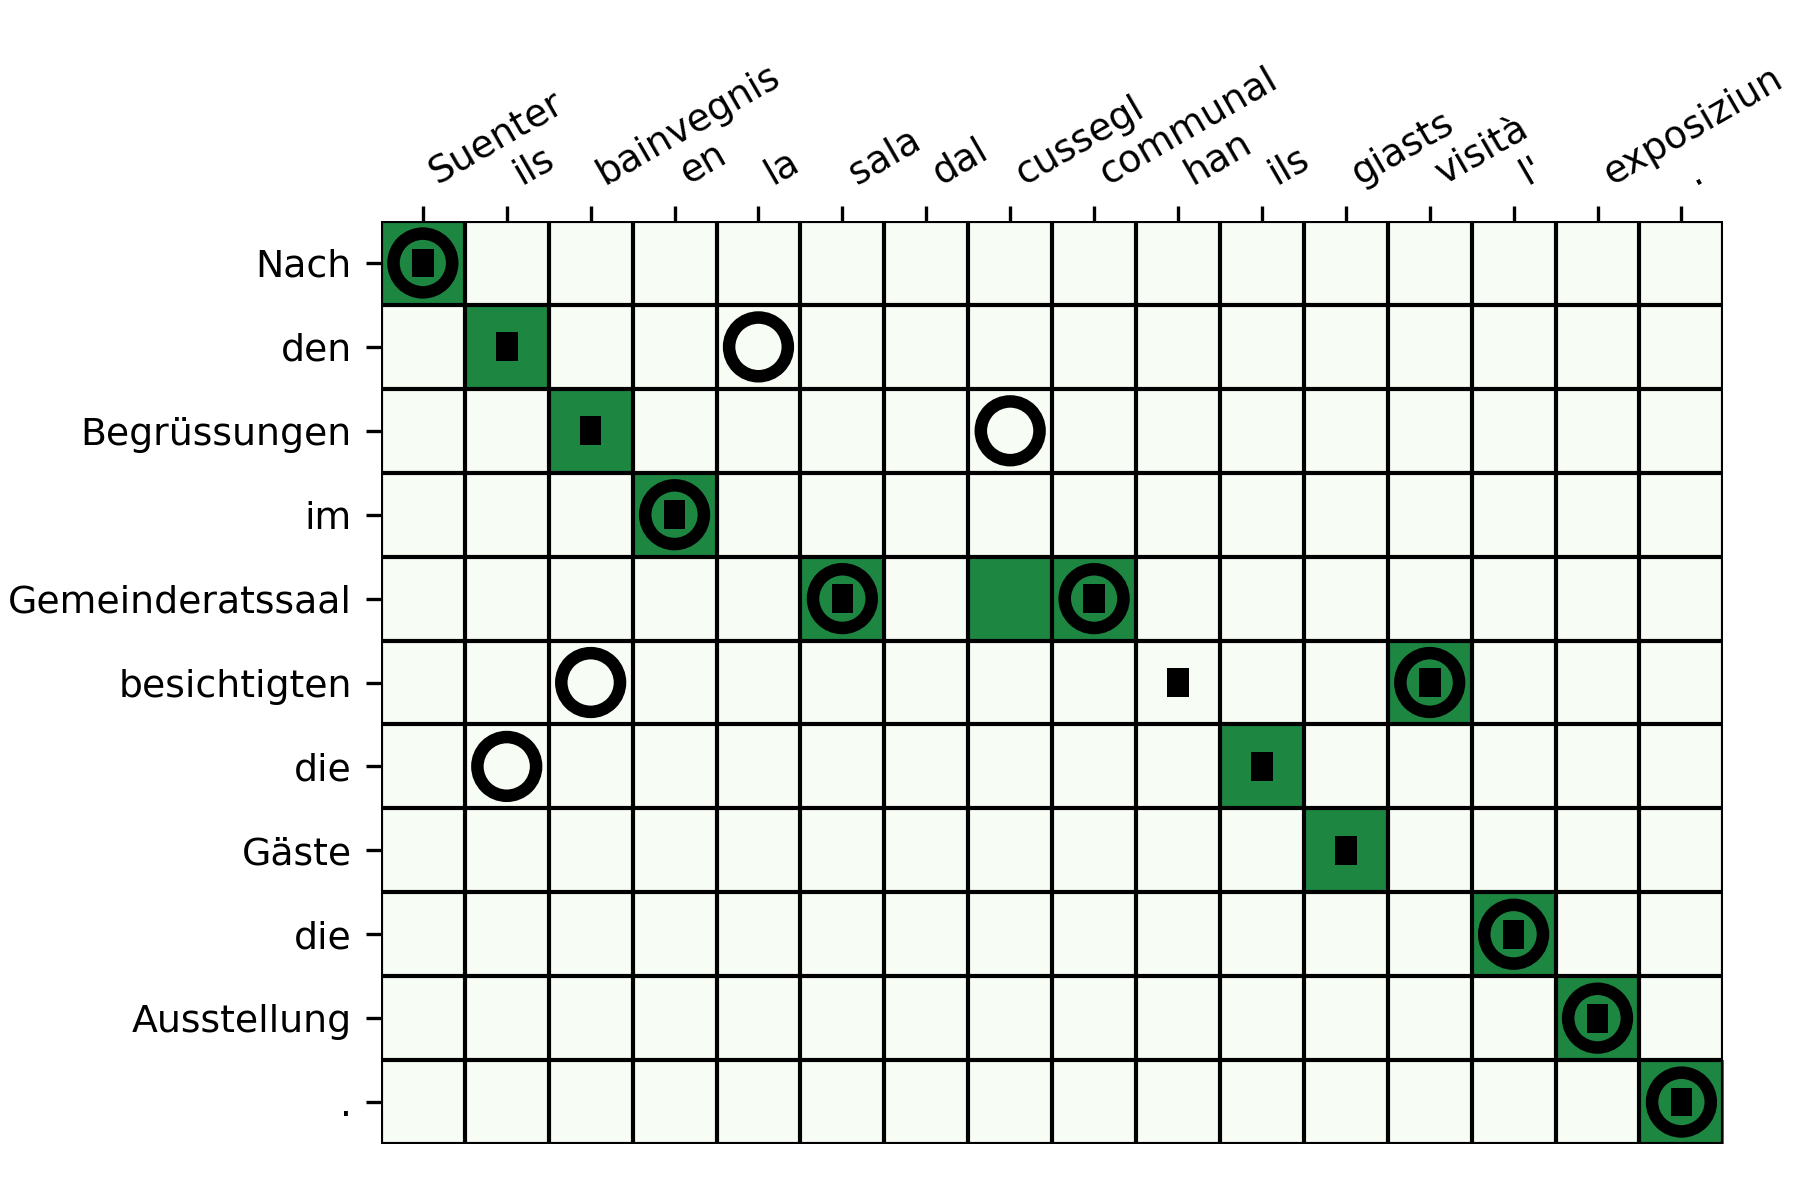
\includegraphics{graphics/alignments/example3.png}
\caption{Word alignment example for the case of German preterite}\label{fig:pret1}
\end{figure}

\begin{figure}
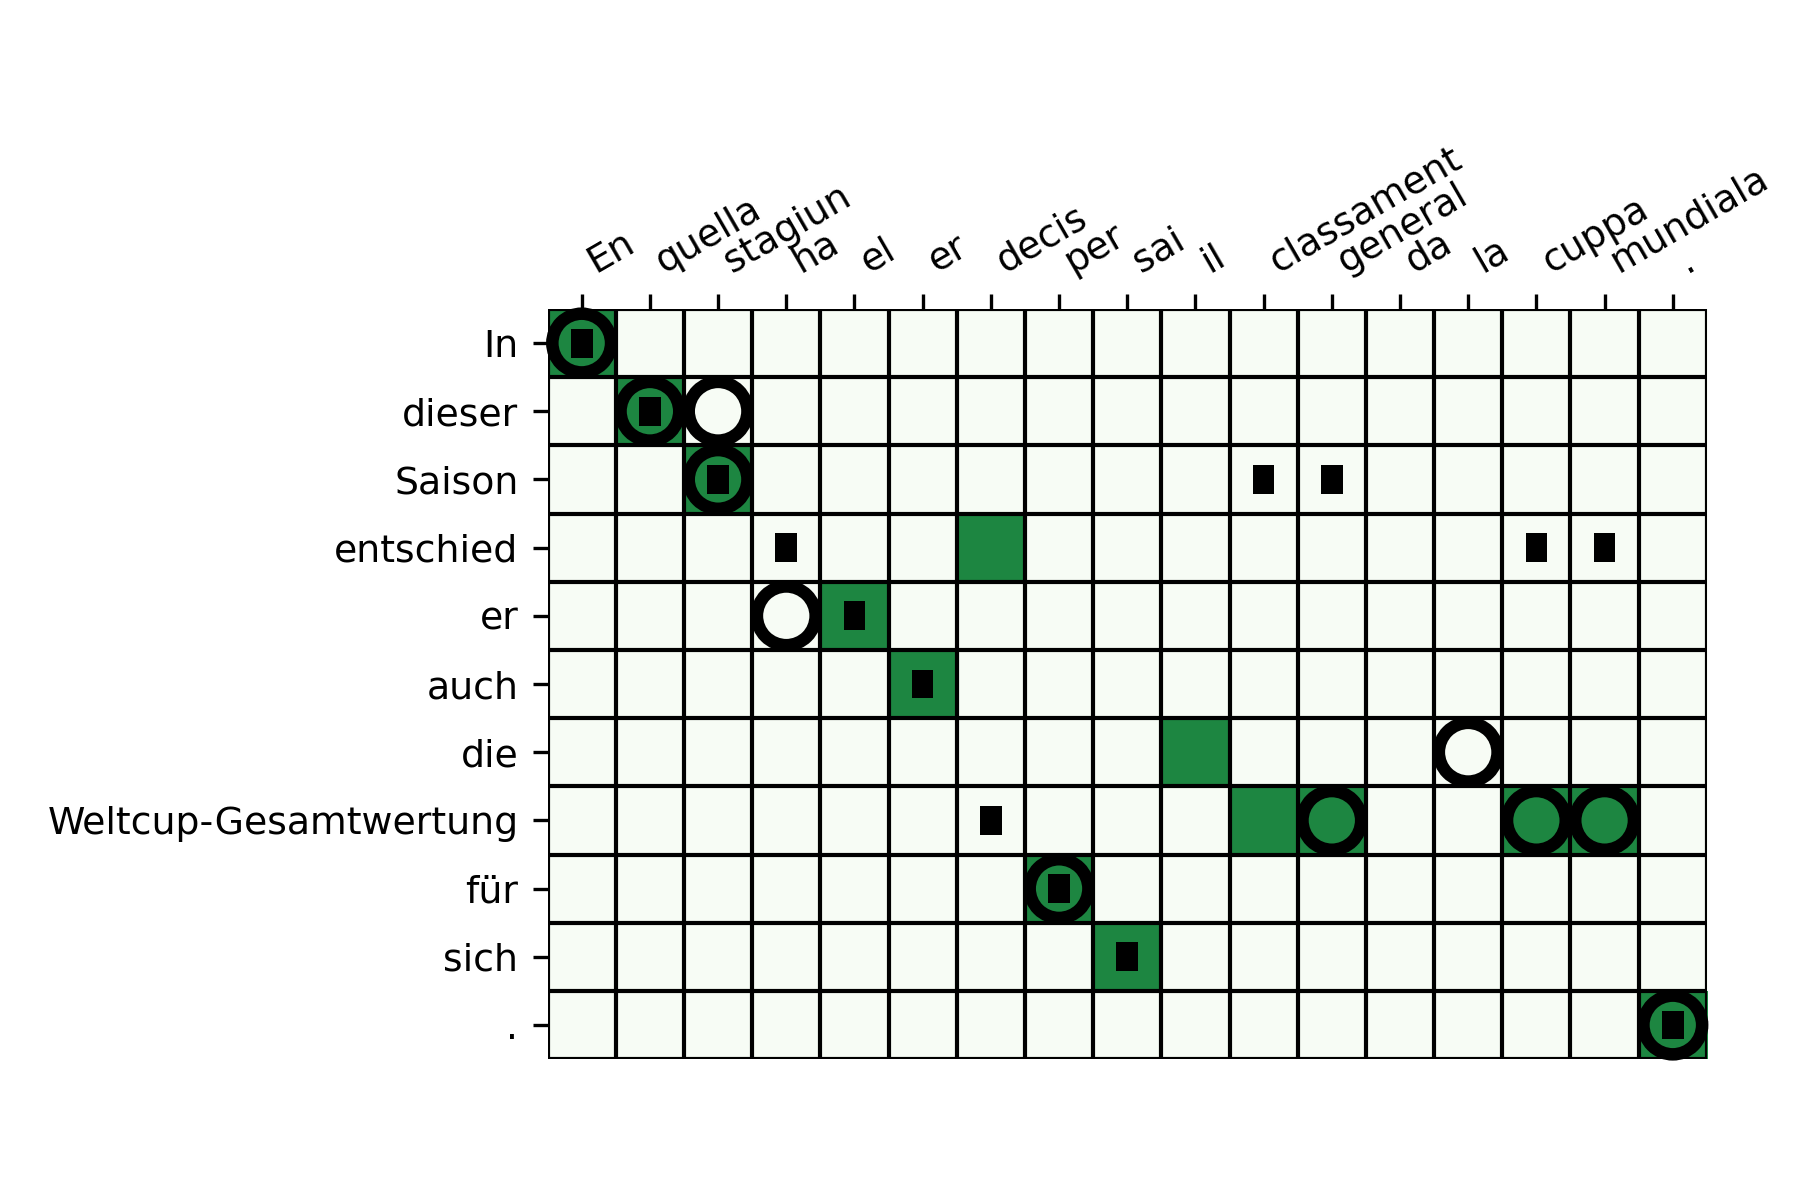
\includegraphics{graphics/alignments/example-pret.png}
\caption{Word alignment example for the case of German preterite}\label{fig:pret2}
\end{figure}

\begin{figure}
	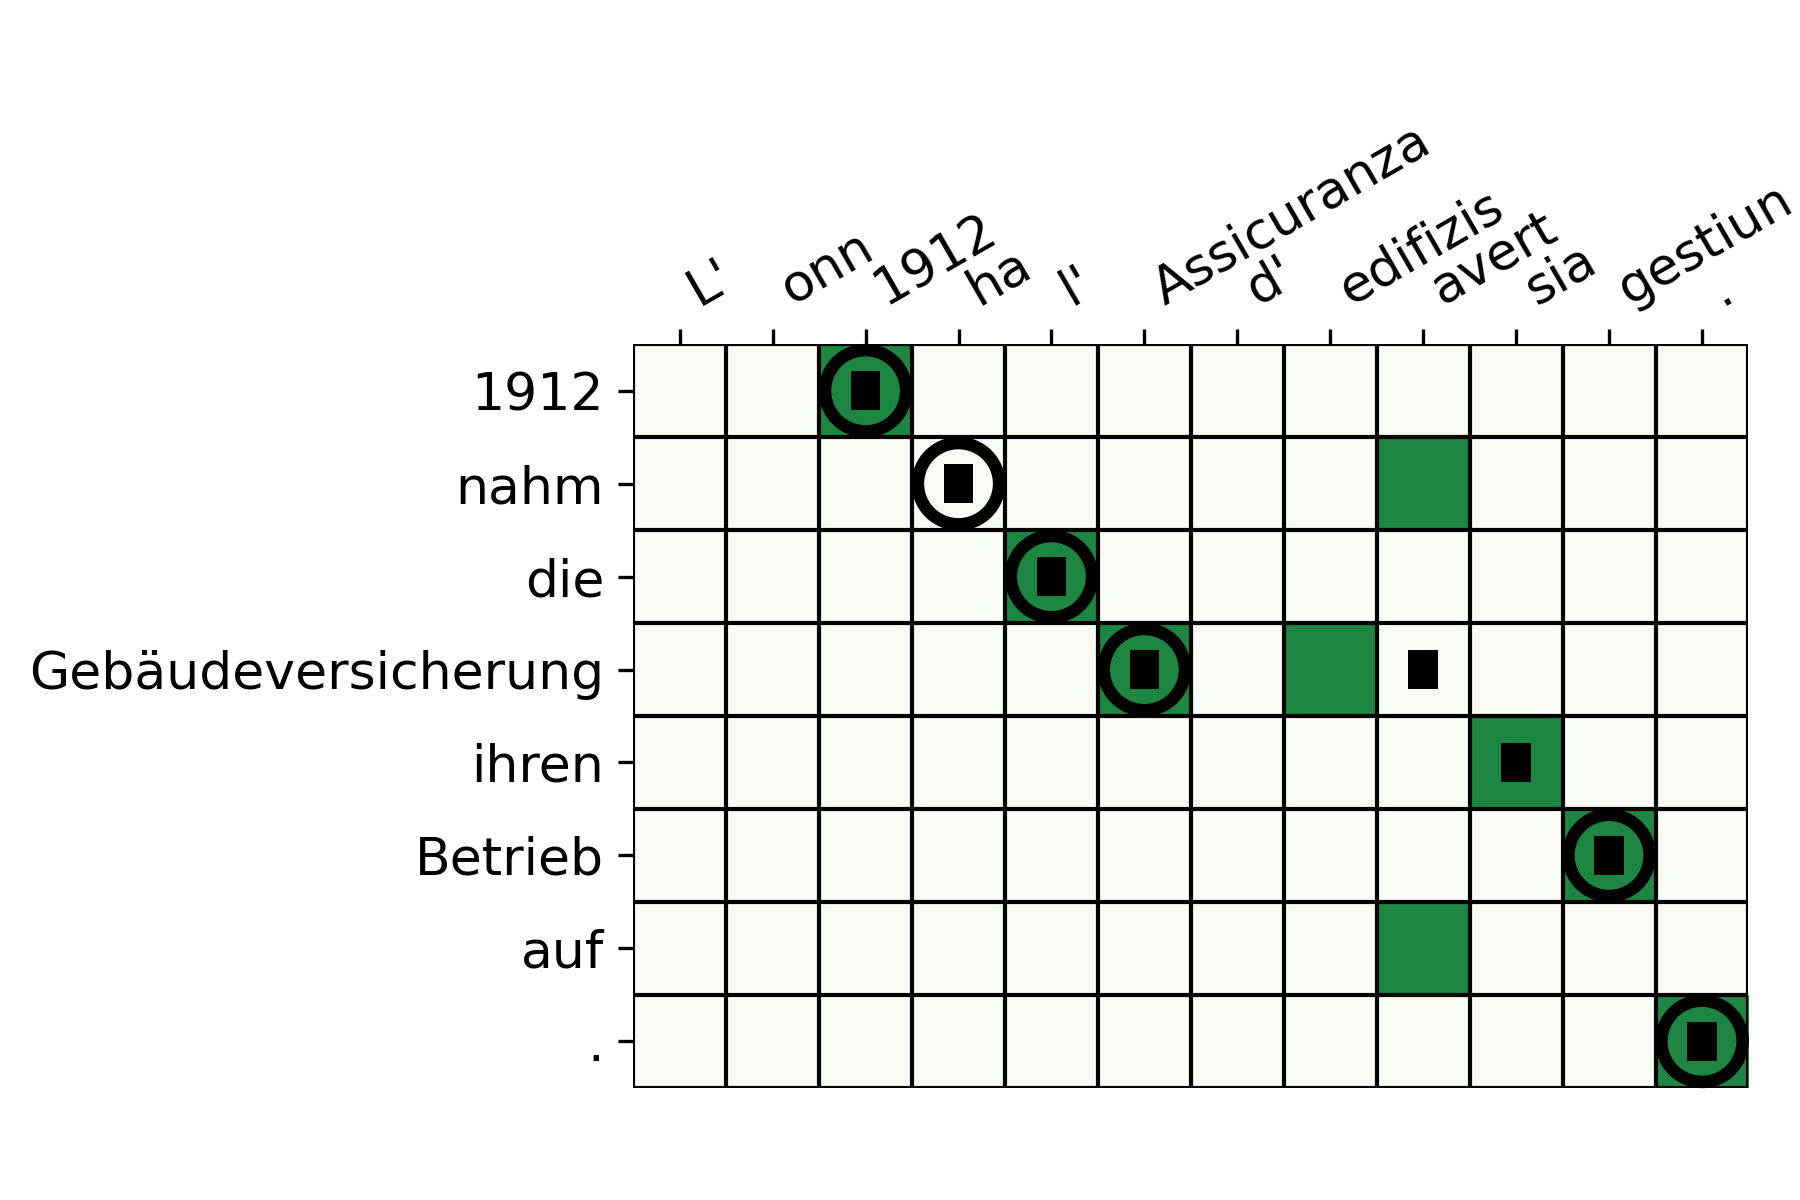
\includegraphics{graphics/alignments/109.png}
	\caption{Word alignment example with a German separable verb in preterite}
	\label{fig:109-1912-nahm}
\end{figure}


\section{Double Negation}
I picked two random cases with negation, which are expressed by the words \emph{na ... 
betg} in Romansh. 
In both cases, (Examples~\ref{fig:na-betg1} and \ref{fig:na-betg2}), eflomal aligns \emph{betg} to the German negation \emph{nicht}, which is correct, but also aligns \emph{na} to the German finite verb, which is wrong. 
SimAlign fails in both cases to align any of the negating words to each other.

\begin{figure}
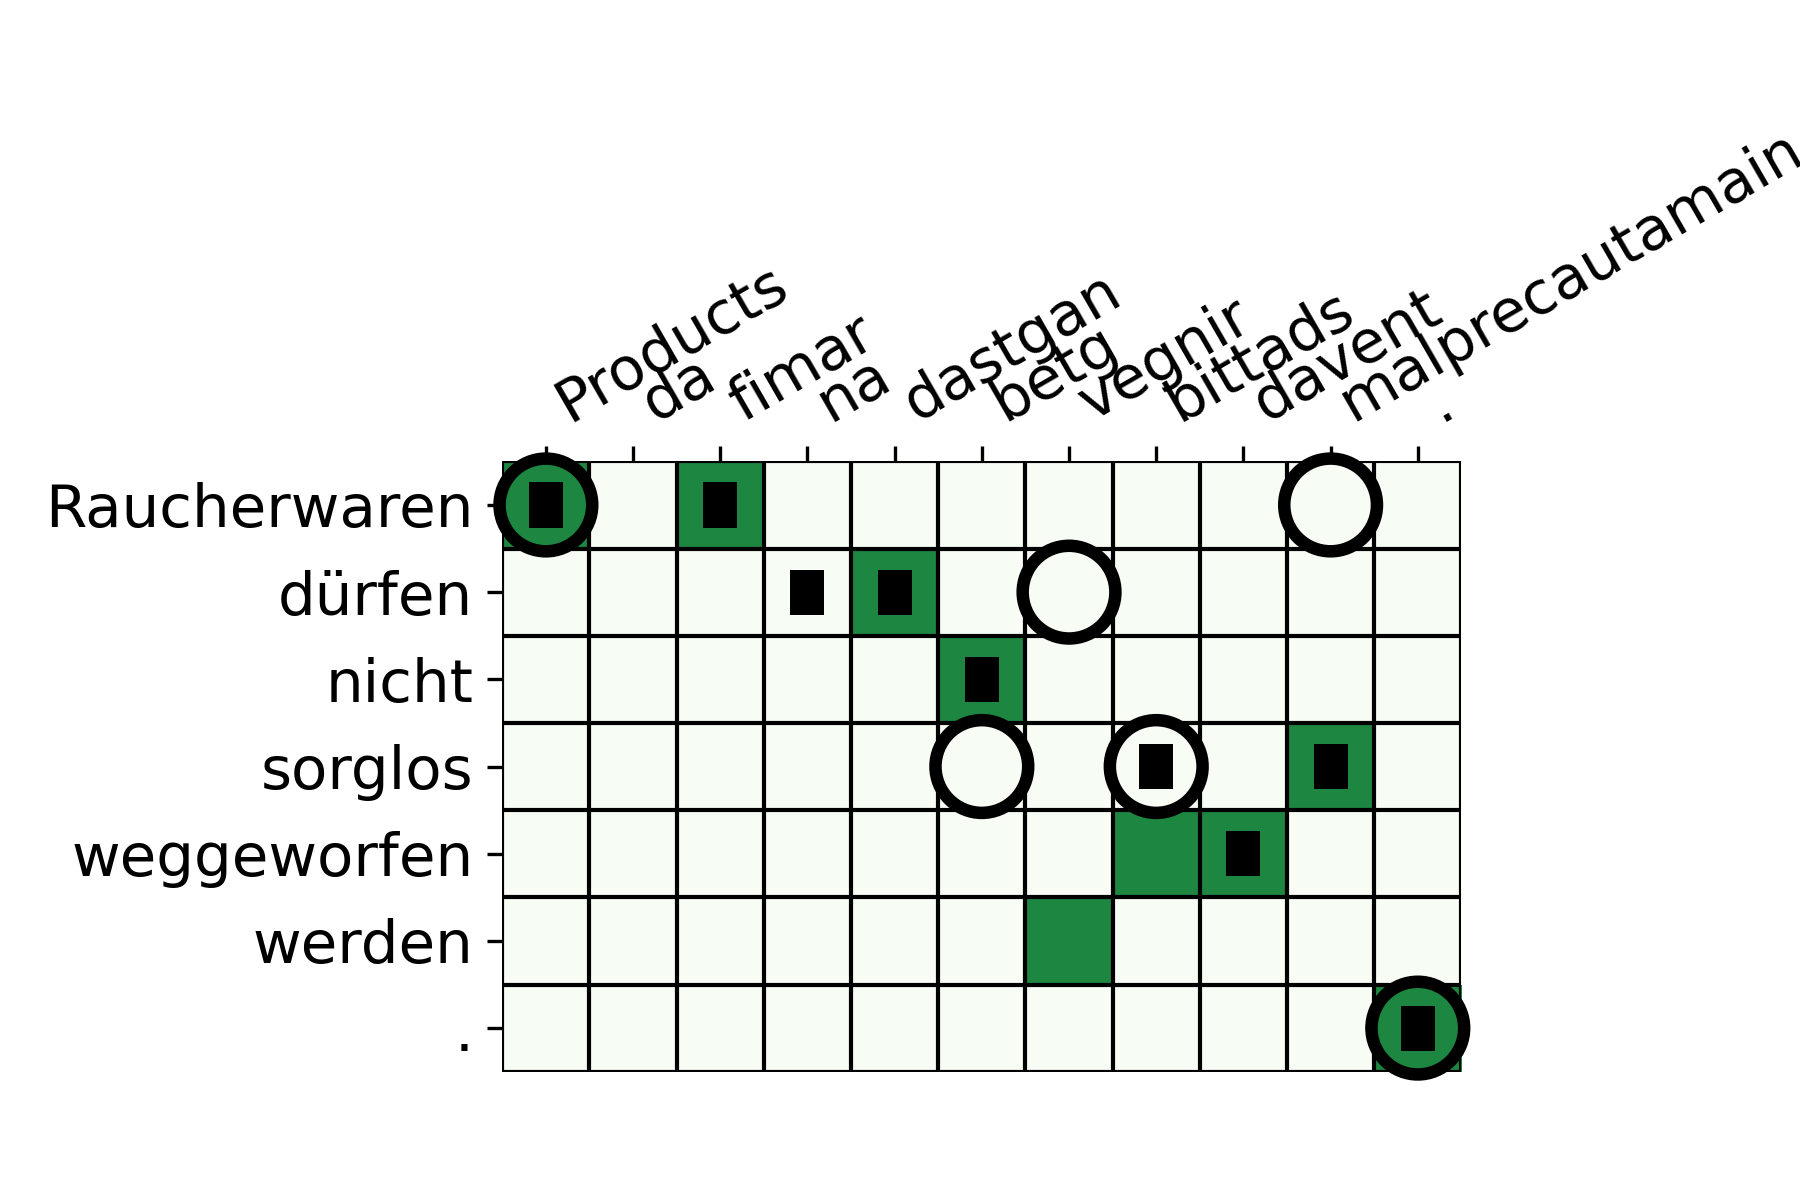
\includegraphics{graphics/alignments/example5.png}
\caption{Word alignment example with Romansh double negation (\emph{na ... 
betg})}
\label{fig:na-betg1}
\end{figure}

\begin{figure}
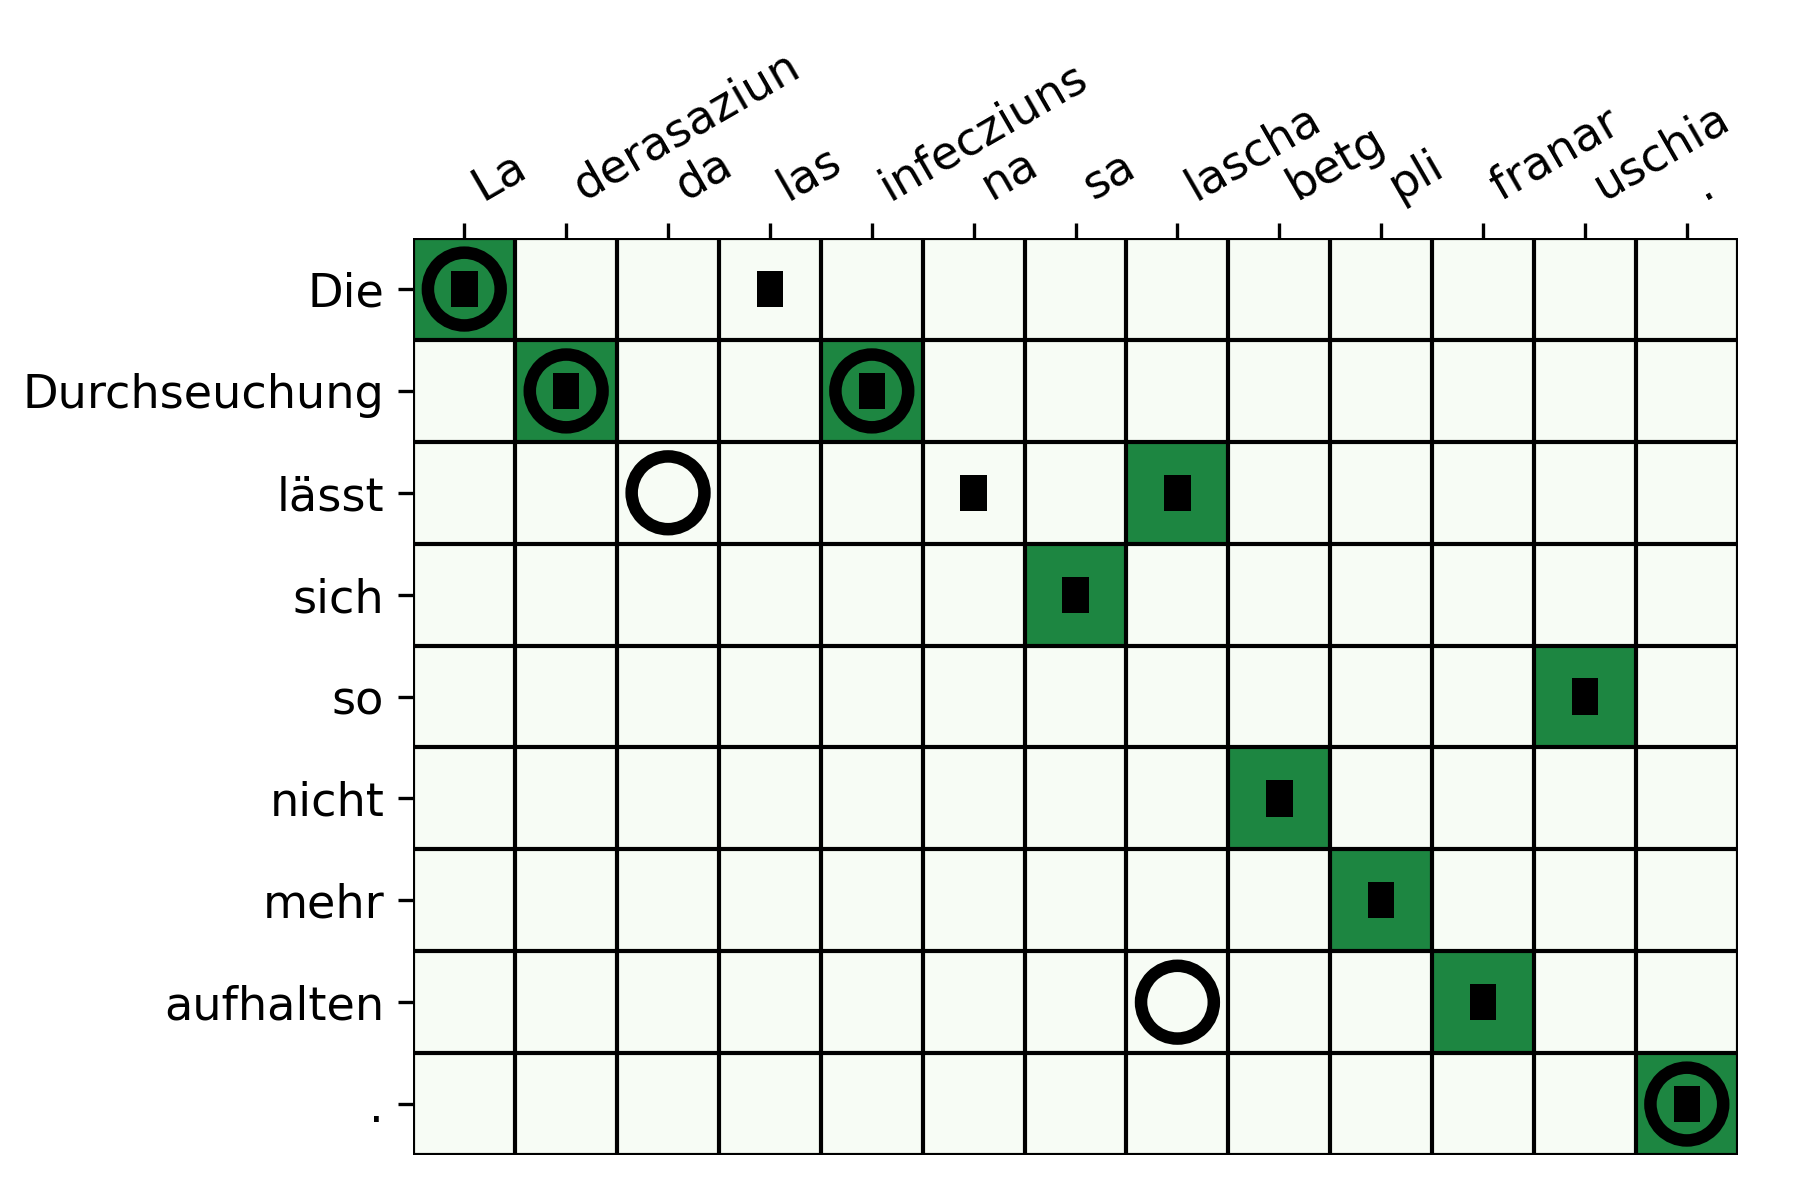
\includegraphics{graphics/alignments/example6-na_betg.png}
\caption{Word alignment example with Romansh double negation (\emph{na ... 
betg})}
\label{fig:na-betg2}
\end{figure}

\section{Differing Word Order}
It seems that both models perform well also when word order differs between German and Romansh. 
In Example~\ref{fig:380-in-graubuenden}, SimAlign has a recalls and precision of 100\%, but eflomal is not far behind, missing only one alignment, namely the past participle (see also Section~\ref{sec:perfect-perfect}).

In Example~\ref{fig:232-mit-einem}, both models deal well with the differing word order, although eflomal's recall is higher. 
Here, eflomal aligns German \emph{möglichst} (\enquote{as much as possible})  to Romansh \emph{tant sco pussaivel}, \emph{correctly} creating a 1-to-many alignment. 
elfomal's precision is punished here due to my gold standard not having Possible alignments for this case of 1-to-many alignment (see also Section~\ref{sec:problems-evaluation}). 

\begin{figure}
	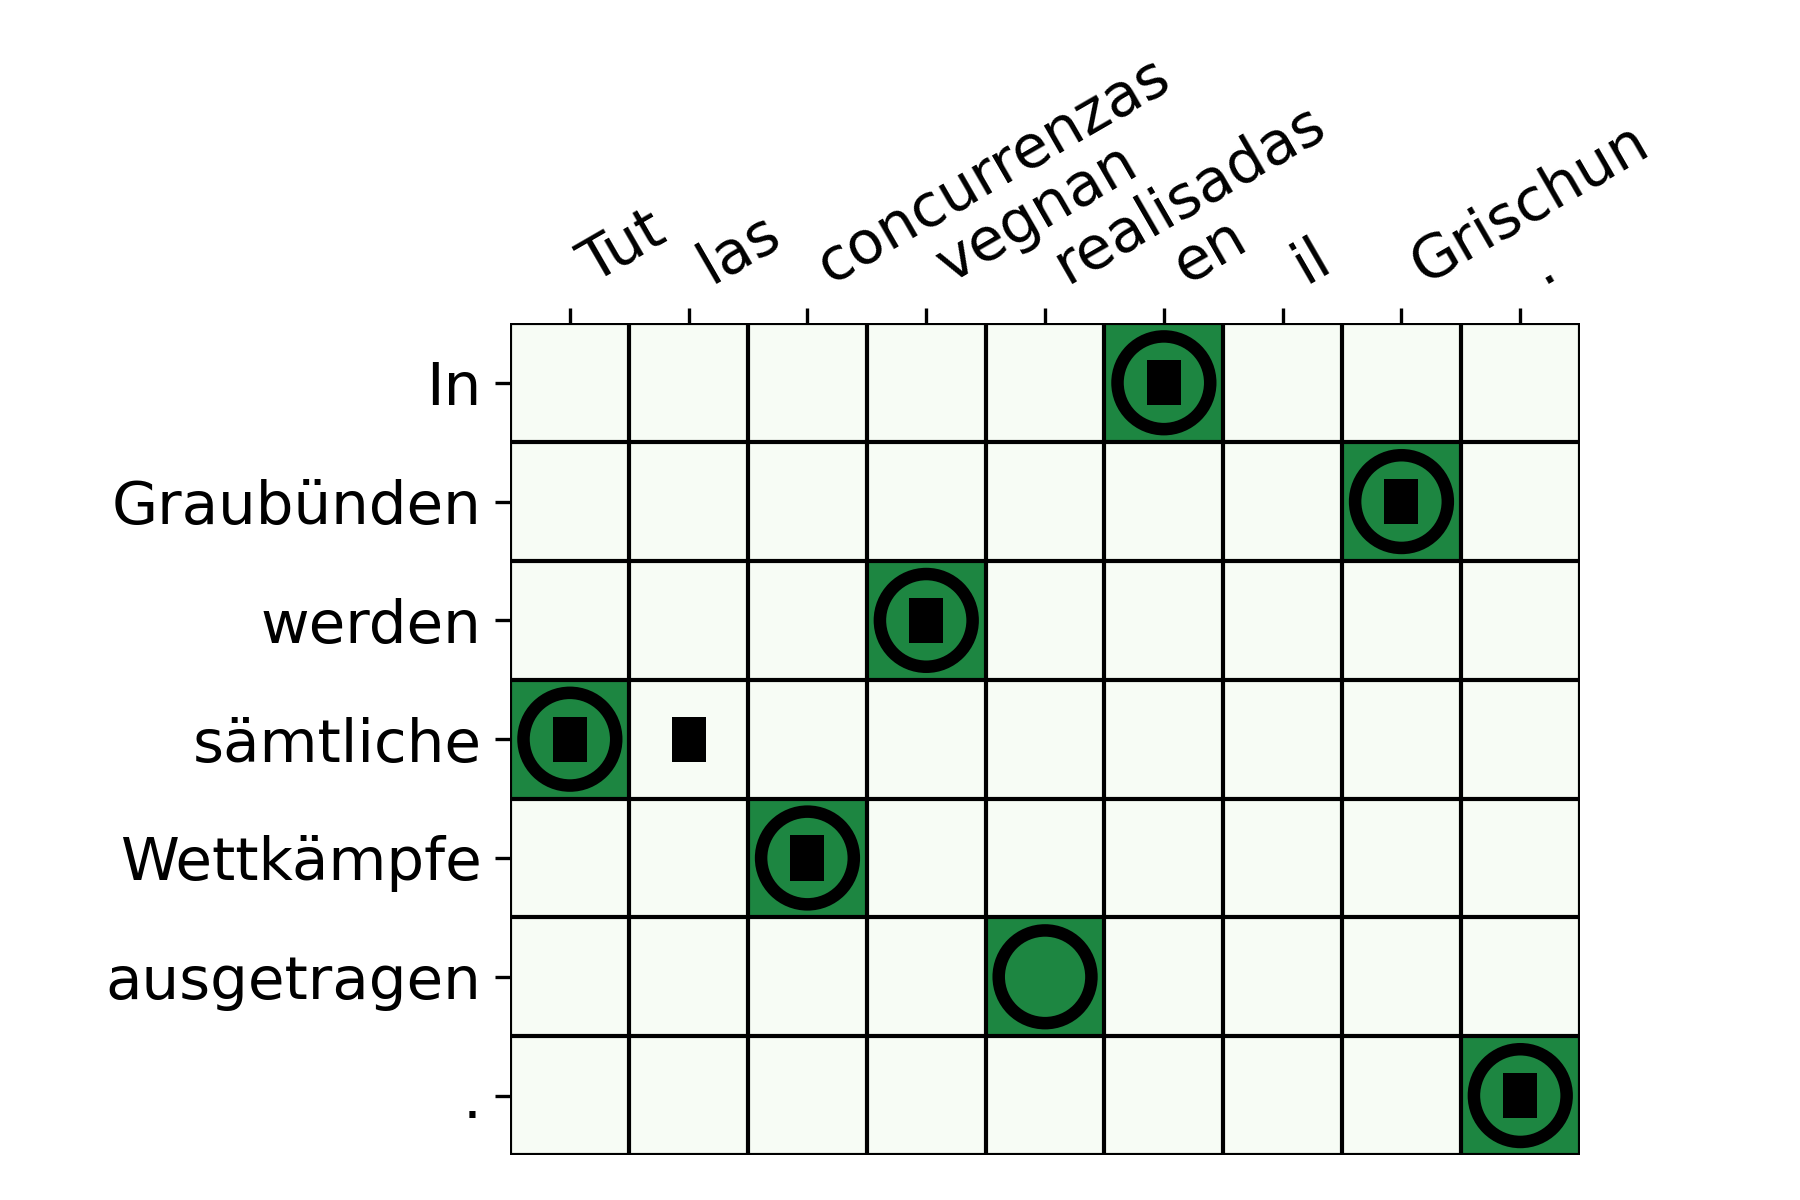
\includegraphics{graphics/alignments/380.png}
	\caption{Word alignment example with differing word order}
	\label{fig:380-in-graubuenden}
\end{figure}


\begin{figure}
	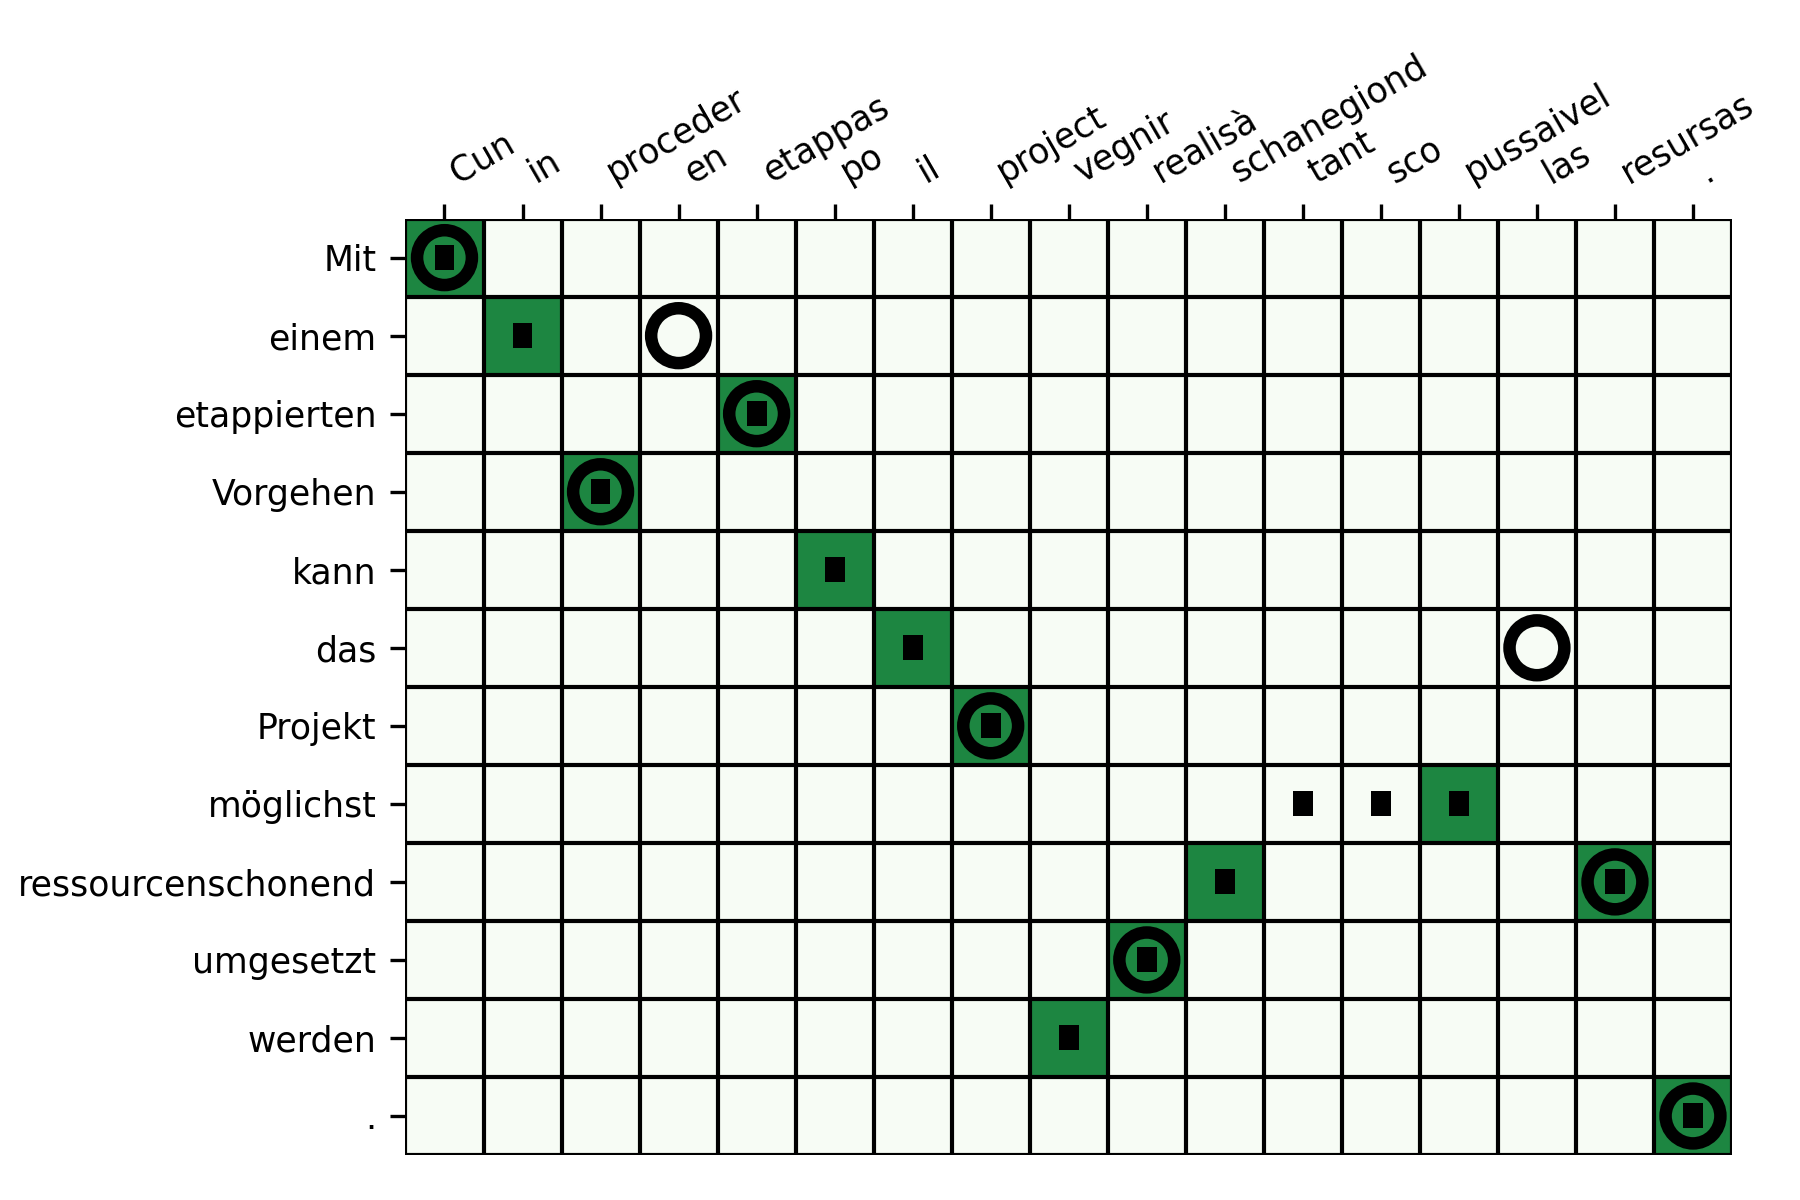
\includegraphics{graphics/alignments/232.png}
	\caption{Word alignment example for a long sentence with differing word order}
	\label{fig:232-mit-einem}
\end{figure}



\begin{figure}
	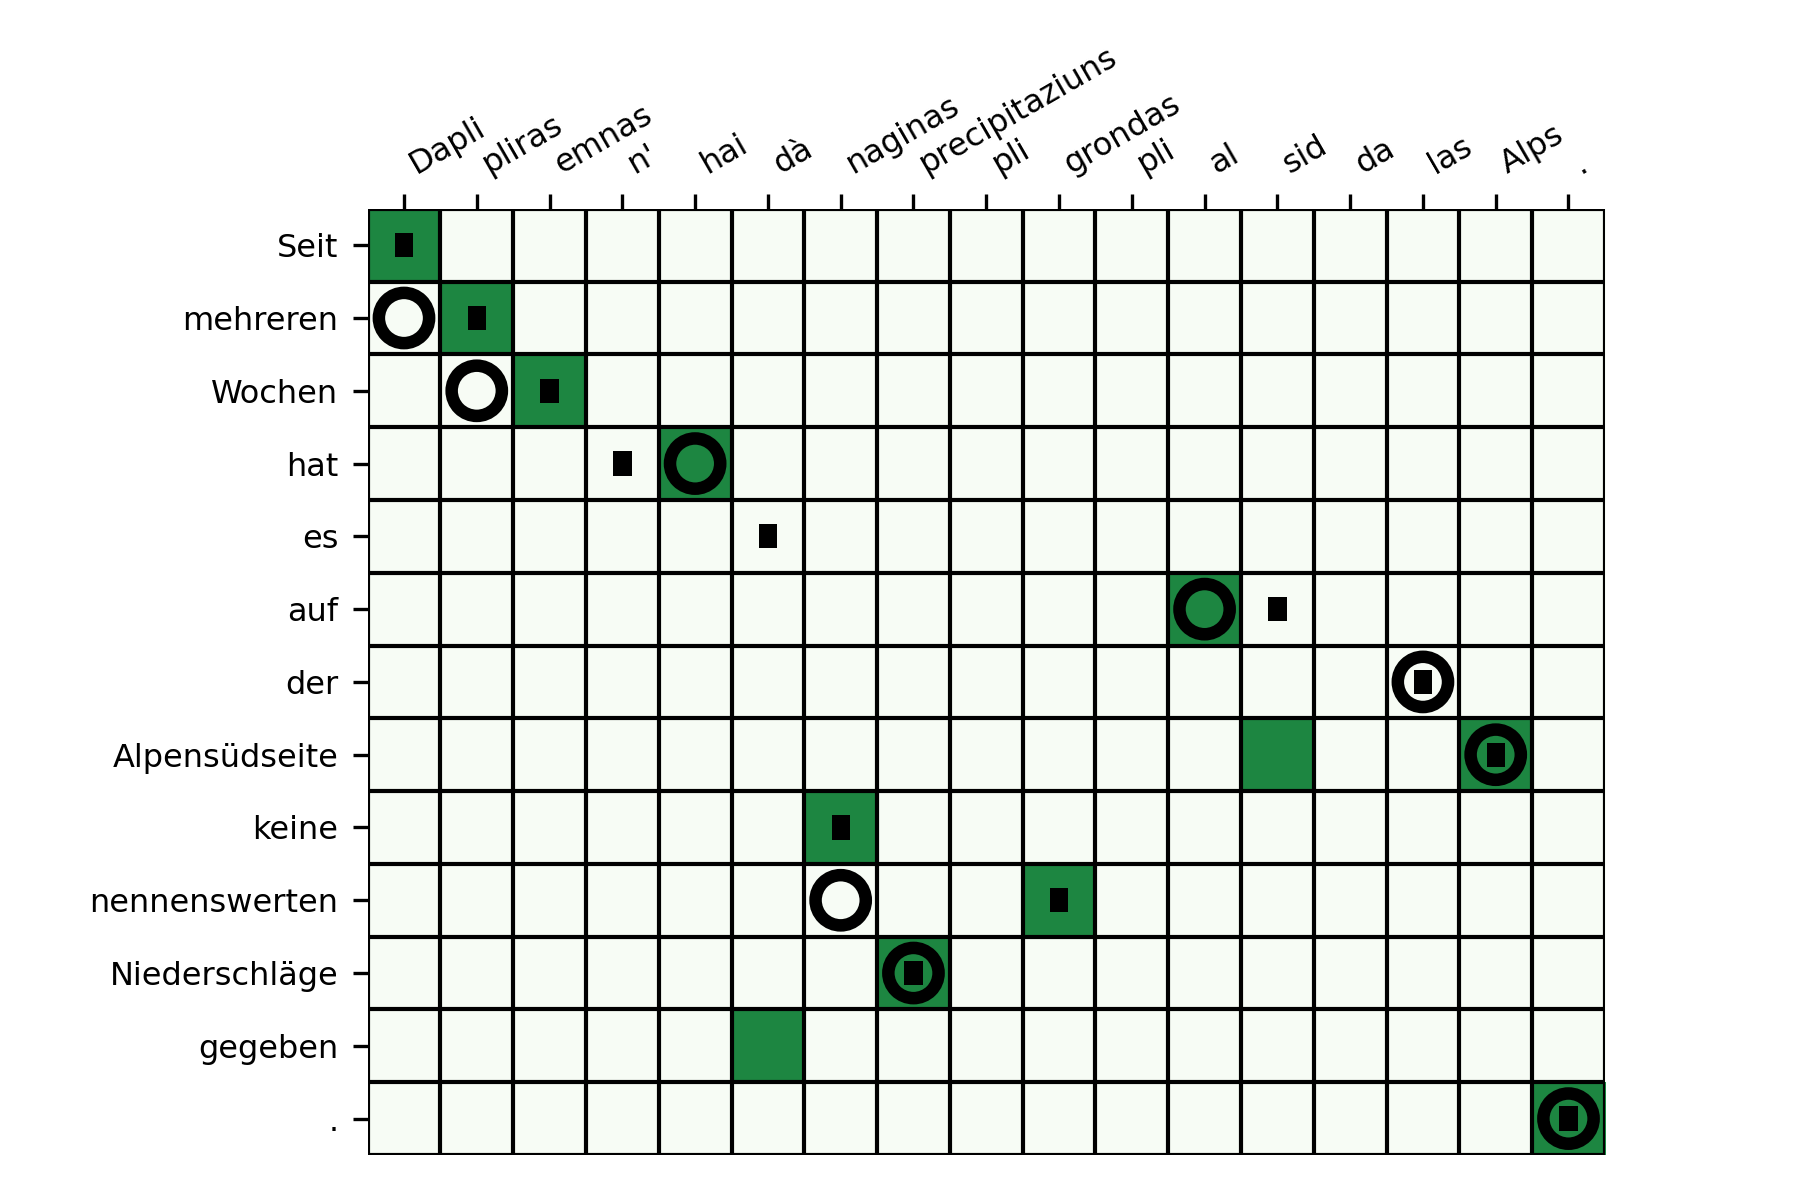
\includegraphics{graphics/alignments/195.png}
	\caption{Word alignment example for a long sentence with differing word order}
	\label{fig:195-seit-mehreren}
\end{figure}

\section{Summary}
I reviewed the differences between eflomal and SimAlign in some specific cases. 
It generally seems that both models perform quite well when German and Romansh follow the same word order and when the sentences mostly contain 1-to-1 alignments. 
German compounds seem to be aligned better by eflomal than by SimAlign. 
Differing word order is more challenging, but is manageable by both models. 
However, the combination of 1-to-many alignments and differing word order seems to be quite challenging for both models.
